%%%%%%%%%%%%%%%%%%%%%%%%%%%%%%%%%%%%%%%%%
% Beamer Presentation
% LaTeX Template
% Version 1.0 (10/11/12)
%
% This template has been downloaded from:
% http://www.LaTeXTemplates.com
%
% License:
% CC BY-NC-SA 3.0 (http://creativecommons.org/licenses/by-nc-sa/3.0/)
%
%%%%%%%%%%%%%%%%%%%%%%%%%%%%%%%%%%%%%%%%%

%----------------------------------------------------------------------------------------
%	PACKAGES AND THEMES
%----------------------------------------------------------------------------------------

\documentclass[aspectratio=169]{beamer}

\mode<presentation> {

% The Beamer class comes with a number of default slide themes
% which change the colors and layouts of slides. Below this is a list
% of all the themes, uncomment each in turn to see what they look like.

%\usetheme{default}
%\usetheme{AnnArbor}
%\usetheme{Antibes}
%\usetheme{Bergen}
%\usetheme{Berkeley}
%\usetheme{Berlin}
%\usetheme{Boadilla}
%\usetheme{CambridgeUS}
%\usetheme{Copenhagen}
%\usetheme{Darmstadt}
%\usetheme{Dresden}
%\usetheme{Frankfurt}
%\usetheme{Goettingen}
%\usetheme{Hannover}
%\usetheme{Ilmenau}
%\usetheme{JuanLesPins}
%\usetheme{Luebeck}
\usetheme{Madrid}
%\usetheme{Malmoe}
%\usetheme{Marburg}
%\usetheme{Montpellier}
%\usetheme{PaloAlto}
%\usetheme{Pittsburgh}
%\usetheme{Rochester}
%\usetheme{Singapore}
%\usetheme{Szeged}
%\usetheme{Warsaw}

% As well as themes, the Beamer class has a number of color themes
% for any slide theme. Uncomment each of these in turn to see how it
% changes the colors of your current slide theme.

%\usecolortheme{albatross}
%\usecolortheme{beaver}
%\usecolortheme{beetle}
%\usecolortheme{crane}
%\usecolortheme{dolphin}
%\usecolortheme{dove}
%\usecolortheme{fly}
%\usecolortheme{lily}
%\usecolortheme{orchid}
%\usecolortheme{rose}
%\usecolortheme{seagull}
%\usecolortheme{seahorse}
%\usecolortheme{whale}
%\usecolortheme{wolverine}

%\setbeamertemplate{footline} % To remove the footer line in all slides uncomment this line
%\setbeamertemplate{footline}[page number] % To replace the footer line in all slides with a simple slide count uncomment this line

%\setbeamertemplate{navigation symbols}{} % To remove the navigation symbols from the bottom of all slides uncomment this line
}

\usepackage{graphicx} % Allows including images
\usepackage{booktabs} % Allows the use of \toprule, \midrule and \bottomrule in tables
\usepackage{amsmath} % Math env.
\usepackage{fontawesome} % Icons for GitHub, etc.
\usepackage{qrcode}
\usepackage{textcomp}


%----------------------------------------------------------------------------------------
%	TITLE PAGE
%----------------------------------------------------------------------------------------

\title[Statistische Geheimhaltung]{Statistische Geheimhaltung - Cell Key Methode} % The short title appears at the bottom of every slide, the full title is only on the title page

\author{Joshua Simon} % Your name
\institute[University Bamberg] % Your institution as it will appear on the bottom of every slide, may be shorthand to save space
{
Otto-Friedrich-University Bamberg \\ % Your institution for the title page
\medskip
\textit{joshua-guenter.simon@stud.uni-bamberg.de} % Your email address
}
\date{May 24, 2022} % Date, can be changed to a custom date

\begin{document}

\begin{frame}
\titlepage % Print the title page as the first slide
\end{frame}

\begin{frame}
\frametitle{Inhalt} % Table of contents slide, comment this block out to remove it
\tableofcontents % Throughout your presentation, if you choose to use \section{} and \subsection{} commands, these will automatically be printed on this slide as an overview of your presentation
\end{frame}


%----------------------------------------------------------------------------------------
%	PRESENTATION SLIDES
%----------------------------------------------------------------------------------------

%------------------------------------------------
\section{Einführung} 
%------------------------------------------------

\subsection{Veröffentlichungen in der amtlichen Statistik}

\begin{frame}{}
    \frametitle{Veröffentlichungen in der amtlichen Statistik}
    \begin{itemize}
        \item Das Ziel der amtlichen Statistik ist die Veröffentlichung von aufbereiteten Information und Daten für Bürger und andere Institutionen
        \item Ein Großteil dieser Veröffentlichungen sind selbst (oder beinhalten) statistische Tabellen aus den amtlichen Daten
    \end{itemize}
\end{frame}


%------------------------------------------------
\subsection{Warum ist Geheimhaltung notwendig?}

\begin{frame}{}
    \frametitle{Warum ist Geheimhaltung notwendig? - I}
    \begin{itemize}
        \item Im deutschen Grundgesetz beschreibt Artikel 2 die Grundlage für ein Recht auf \textbf{informationelle Selbstbestimmung} - das Fundament unseres modernen Datenschutzes
        \item Die amtliche Statistik kommt dieser Verantwortung mit dem \textbf{Statistikgeheimnis} (§ 16 Abs. 1 Satz 1 BStatG) nach: \\
        \textit{„Einzelangaben über persönliche und sachliche Verhältnisse, die für eine Bundesstatistik
        gemacht werden, sind von den Amtsträgern und für den öffentlichen Dienst besonders
        Verpflichteten, die mit der Durchführung von Bundesstatistiken betraut sind, geheim zu halten,
        soweit durch besondere Rechtsvorschrift nichts anderes bestimmt ist.“}
    \end{itemize}
\end{frame}


\begin{frame}{}
    \frametitle{Warum ist Geheimhaltung notwendig? - II}
    Konkret möchte man mit der statistischen Geheimhaltung die Folgende Punkte bedienen (nach Begründung zum BStatG; BT-Drucks. Nr. 10/5345 vom 17. April 1986) \cite{Nickl}:
    \begin{itemize}
        \item Schutz von einzelnen Personen und Entitäten vor der Offenlegung ihrer sensitiven Daten
        \item Aufrechterhaltung des Vertrauensverhältnisses zwischen den Befragten und den statistischen Ämtern und erhebenden Einrichtungen
        \item Gewährleistung der Zuverlässigkeit der Angaben und der Berichswilligkeit der Befrageten
    \end{itemize}
\end{frame}


\begin{frame}{}
    \frametitle{Warum ist Geheimhaltung notwendig? - III}
    An manche Stellen erlauben Ausnahmen, die Geheimhaltung auszusetzen. Hier sind beispielsweise die folgenden Stellen betroffen \cite{Nickl}:
    \begin{itemize}
        \item Wenn Befragte explizit einer Veröffentlichung von Einzelangaben zustimmen
        \item Wenn sich Informationen aus allgemein zugänglichen Quellen von öffentlichen Stellen beziehen
        \item Absolut anonyme Einzeldaten oder zusammengefasste Einzeldaten (statistischen Ergebnisse)
        \item Weitere Ausnahmen zur behördlichen Übermittlung, Methodenentwicklung, Planungs- und Forschungszwecke sind über das BStatG geregelt
    \end{itemize}
\end{frame}


%------------------------------------------------
\section{Etablierte Geheimhaltungsverfahren}
%------------------------------------------------

\begin{frame}{}
	\frametitle{Etablierte Geheimhaltungsverfahren}
    \begin{center}
        \huge Etablierte Geheimhaltungsverfahren
    \end{center}
\end{frame}


\begin{frame}
    \frametitle{Etablierte Geheimhaltungsverfahren}
    Bei den verfügbaren Geheimhaltungsverfahren unterscheidt man zunächst zwischen:
    \begin{itemize}
        \item \textbf{Informationsreduzierende Methoden}: Hier werden durch Aggregation (Zusammenfassen) oder Sperrung/Löschung kritischer Kategrorien oder Werte die Aufdeckungsrisiken verhindert.
        \item \textbf{Datenverändernde Methoden}: Hier werden durch gezielte Veränderungen der Daten - z.B. durch Runden oder Zufallsüberlagerungen - kritsiche Werte verfälscht.
    \end{itemize}
\end{frame}


%------------------------------------------------
\subsection{Pre-tabulare und post-tabulare Verfahren}

\begin{frame}
    \frametitle{Pre-tabulare und post-tabulare Verfahren}
    Weiter unterscheidt man Geheimhaltungsverfahren auch nach dem Zeitpunkt ihrer Durchführung:
    \begin{itemize}
        \item \textbf{Pre-tabulare Verfahren}: Bei diesen Verfahren spricht man oft auch von einer Anonymisierung, da die Daten bereits vor der Tabellierung so verändert werden, dass keine kritschen Ergebnisse resultieren. Oftmals ist diese Art von Geheimhaltung aber nicht ausreichend, weshalb weitere Verfahren im Anschluss angewandt werden müssen.
        \item \textbf{Post-tabulare Verfahren}: Diese Verfahren werden erst im Anschluss an die Tabellierung der Daten angewandt.
    \end{itemize}
\end{frame}


%------------------------------------------------
\subsection{Häufigkeits- und Wertetabellen}

\begin{frame}
    \frametitle{Häufigkeits- und Wertetabellen - I}
    Maßgebend für die Anwendung eines Geheimhaltungsverfahren ist die Art der zu veröffentlichenden Tabelle, die vorliegt. Man unterscheidet zwischen:
    \begin{itemize}
        \item \textbf{Häufigkeitstabellen}: Stellen Häufigkeiten oder Fallzahlen dar, z.B. Anzahl von Frauen und Männern innerhalb einer Universität.
        \item \textbf{Wertetabellen}: Stellen Wertesummen dar, z.B. Umsätze.
    \end{itemize}
\end{frame}


\begin{frame}
    \frametitle{Häufigkeits- und Wertetabellen - II}
    Für diese beiden Tabellentypen stehen eine Reihe an Geheimhaltungsregeln zur Verfügung, die beschreiben, wenn ein Geheimhaltungsverfahren angewandt werden muss \cite{Nickl}.
    \begin{center}
        \begin{tabular}{ r r }
         \textbf{Tabellenart} \vline & \textbf{Geheimhaltungsregeln} \\ 
         \hline
         \textbf{Häufigkeitstabellen} \vline & Mindestfallzahlregel, Randwertregel \\  
         \vline & \\
         \hline
         \textbf{Wertetabellen} \vline & Dominanz-Konzentrationsregeln:  \\
         \vline & $(1,k)$-Regel, $2,(k)$-Regel, $p$\%-Regel, \\
         \vline & Fallzahlregel
        \end{tabular}
    \end{center}
\end{frame}


\begin{frame}
    \frametitle{Häufigkeits- und Wertetabellen - II}
    Für diese beiden Tabellentypen stehen eine Reihe an Geheimhaltungsregeln zur Verfügung, die beschreiben, wenn ein Geheimhaltungsverfahren angewandt werden muss \cite{Nickl}.
    \begin{center}
        \begin{tabular}{ r r }
         \textbf{Tabellenart} \vline & \textbf{Geheimhaltungsregeln} \\ 
         \hline
         \textbf{Häufigkeitstabellen} \vline & \textcolor{blue}{Mindestfallzahlregel}, Randwertregel \\  
         \vline & \\
         \hline
         \textbf{Wertetabellen} \vline & Dominanz-Konzentrationsregeln:  \\
         \vline & $(1,k)$-Regel, $2,(k)$-Regel, \textcolor{blue}{$p$\%-Regel}, \\
         \vline & Fallzahlregel
        \end{tabular}
    \end{center}
    Die in \textcolor{blue}{blau} gekennzeichneten Verfahren werden hier genauer beleuchtet.
\end{frame}


%------------------------------------------------
\subsection{Ausgewählte Verfahren}

\begin{frame}
    \frametitle{Mindestfallzahlregel}
    \begin{theorem}[Mindestfallzahlregel]
        Ein Tabellenfeld bzw. eine Zelle $c$ wird genau dann geheim gehalten, wenn weniger als $n$ Einheiten darin enthalten sind, also $c < n$ gilt.
    \end{theorem}
    In vielen Statistiken wird $n = 3$ gewählt, d.h. Zellenwerte kleiner als $3$ drüfen nicht veröffentlicht werden \cite{Nickl}.
\end{frame}


\begin{frame}
    \frametitle{Mindestfallzahlregel - Zellsperrung I}
    Nach Feststellung der kritischen Werte in einer Häufigkeitstabelle, kann ein Geheimhaltungsverfahren angewandt werden. Die verbreiteste Methode ist dabei die Zellsperrung \cite{Rothe-1}, \cite{Nickl}.
    \begin{theorem}[Zellsperrung]
        Die Zellsperrung setzt sich aus zwei Schritten zusammen:
        \begin{enumerate}
            \item \textbf{Primärsperrung}: Die anhand der Mindestfallzahlregel ermittelten kritsichen Werte werden durch ein "x" ersetzt.
            \item \textbf{Sekundärsperrung}: Um Rückrechnungen zu vermeiden, werden 3 weitere Zellen der Tabelle mit "x" ersetzt.
        \end{enumerate}
    \end{theorem}
    Beim Ersetzen eines Tabellenfeldes durch "x" spricht man auch von einer Sperrung oder Zellsperrung.
\end{frame}


\begin{frame}
    \frametitle{Mindestfallzahlregel - Zellsperrung II}
    Folgendes Beispiel soll die Anwendung der Zellsperrung illustieren. \\
    \textcolor{red}{Anwendung der Mindestfallzahlregel für $n = 3$}
    \begin{center}
        \begin{tabular}{ r r r r }
         \textbf{Studienfach} \vline & \textbf{männlich} & \textbf{weiblich} & \textbf{insgesamt} \\ 
         \hline
         Bauingenieurwesen \vline & $4$ & $3$ & $7$ \\
         Informatik \vline & $9$ & $12$ & $21$ \\  
         Medizin \vline & $4$ & $\textcolor{red}{1}$ & $5$ \\
         Survey Statistik \vline & $10$ & $10$ & $20$ \\
         \hline
         Gesamt \vline & $27$ & $26$ & $53$
        \end{tabular}
    \end{center}
\end{frame}


\begin{frame}
    \frametitle{Mindestfallzahlregel - Zellsperrung III}
    Folgendes Beispiel soll die Anwendung der Zellsperrung illustieren. \\
    \textcolor{red}{Anwendung der Primärsperrung}
    \begin{center}
        \begin{tabular}{ r r r r }
         \textbf{Studienfach} \vline & \textbf{männlich} & \textbf{weiblich} & \textbf{insgesamt} \\ 
         \hline
         Bauingenieurwesen \vline & $4$ & $3$ & $7$ \\
         Informatik \vline & $9$ & $12$ & $21$ \\  
         Medizin \vline & $4$ & \textcolor{red}{x} & $5$ \\
         Survey Statistik \vline & $10$ & $10$ & $20$ \\
         \hline
         Gesamt \vline & $27$ & $26$ & $53$
        \end{tabular}
    \end{center}
\end{frame}


\begin{frame}
    \frametitle{Mindestfallzahlregel - Zellsperrung IV}
    Folgendes Beispiel soll die Anwendung der Zellsperrung illustieren. \\
    \textcolor{red}{Anwendung der Sekundärsperrung}
    \begin{center}
        \begin{tabular}{ r r r r }
         \textbf{Studienfach} \vline & \textbf{männlich} & \textbf{weiblich} & \textbf{insgesamt} \\ 
         \hline
         Bauingenieurwesen \vline & $\textcolor{red}{4}$ & $\textcolor{red}{3}$ & $7$ \\
         Informatik \vline & $9$ & $12$ & $21$ \\  
         Medizin \vline & $\textcolor{red}{4}$ & \textcolor{red}{x} & $5$ \\
         Survey Statistik \vline & $10$ & $10$ & $20$ \\
         \hline
         Gesamt \vline & $27$ & $26$ & $53$
        \end{tabular}
    \end{center}
\end{frame}


\begin{frame}
    \frametitle{Mindestfallzahlregel - Zellsperrung V}
    Folgendes Beispiel soll die Anwendung der Zellsperrung illustieren. \\
    \textcolor{red}{Anwendung der Sekundärsperrung}
    \begin{center}
        \begin{tabular}{ r r r r }
         \textbf{Studienfach} \vline & \textbf{männlich} & \textbf{weiblich} & \textbf{insgesamt} \\ 
         \hline
         Bauingenieurwesen \vline & \textcolor{red}{x} & \textcolor{red}{x} & $7$ \\
         Informatik \vline & $9$ & $12$ & $21$ \\  
         Medizin \vline & \textcolor{red}{x} & \textcolor{red}{x} & $5$ \\
         Survey Statistik \vline & $10$ & $10$ & $20$ \\
         \hline
         Gesamt \vline & $27$ & $26$ & $53$
        \end{tabular}
    \end{center}
\end{frame}


\begin{frame}
    \frametitle{$p$\%-Regel}
    Die Defintion der folgenden Regel kann in \cite{Rothe-2} gefunden werden.
    \begin{theorem}[$p$\%-Regel]
        Ein Tabellenfeld bzw. eine Zelle $c$ wird genau dann geheim gehalten, wenn die Differenz $d$ zwischen dem Zellwert $c$ und dem zweitgrößten Beitrag $x_2$ den größten Beitrag $x_1$ um weniger als $p$\% übersteigt. Es gilt also 
        \begin{align}
            & d = c - x_2 < x_1 + \frac{p}{100} \cdot x_1 \\
            \Leftrightarrow \: & c - x_2 - x_ 1 <  \frac{p}{100} \cdot x_1.
        \end{align}
    \end{theorem}
    Der Wert $p$ wird dabei statistikspezifisch festgelegt.
\end{frame}


\begin{frame}
    \frametitle{$p$\%-Regel - Beispiel I}
    Die $p$\%-Regel soll am folgenden Beispiel illustieren werden. Gegeben seinen die Umsätze von drei verschiedenen (fiktiven) Bamberger Bierbrauereien.
    \begin{center}
        \begin{tabular}{ r r r r r }
            \textbf{Brauerei} \vline & \textbf{Mährs Bräu} & \textbf{Schinkerla} & \textbf{Käsmann} & \textbf{Gesamt} \\ 
            \hline
            Umsatz \vline & $600.000$ & $50.000$ & $250.000$ & $900.000$
           \end{tabular}
    \end{center}
    Die Anwendung der $p$\%-Regel mit $p = 10 \%$ und Zellenwert $c = 600.000$ liefert hier:
    \begin{itemize}
        \item Größter Beitrag $x_1 = 900.000$
        \item Zweitgrößter Beitrag $x_2 = 250.000$
    \end{itemize}
\end{frame}


\begin{frame}
    \frametitle{$p$\%-Regel - Beispiel II}
    Die $p$\%-Regel soll am folgenden Beispiel illustieren werden. Gegeben seinen die Umsätze von drei verschiedenen (fiktiven) Bamberger Bierbrauereien.
    \begin{center}
        \begin{tabular}{ r r r r r }
            \textbf{Brauerei} \vline & \textbf{Mährs Bräu} & \textbf{Schinkerla} & \textbf{Käsmann} & \textbf{Gesamt} \\ 
            \hline
            Umsatz \vline & $600.000$ & $50.000$ & $250.000$ & $900.000$
           \end{tabular}
    \end{center}
    Die Anwendung der $p$\%-Regel mit $p = 10 \%$ und Zellenwert $c = 600.000$ liefert hier:
    \begin{itemize}
        \item Größter Beitrag $x_1 = 900.000$
        \item Zweitgrößter Beitrag $x_2 = 250.000$
    \end{itemize}
    \begin{align}
        & c - x_2 - x_ 1 <  \frac{p}{100} \cdot x_1 \\
        \Leftrightarrow \: & 900.000 - 250.000 - 600.000 < \frac{10}{100} \cdot 600.000 \\
        \Leftrightarrow \: & 50.000 < 60.000
    \end{align}
    Es folgt, dass der Zellenwert $c$ geheimgehalten werden muss.
\end{frame}


%------------------------------------------------
\section{Cell Key Methode}
%------------------------------------------------

\begin{frame}{}
	\frametitle{Cell Key Methode}
    \begin{center}
        \huge Cell Key Methode
    \end{center}
\end{frame}


%------------------------------------------------
\subsection{Methodik}

\begin{frame}{}
	\frametitle{Cell Key Methode - Facts}
    \begin{itemize}
        \item Die bislang gezeigten Geheimhaltungsverfahren müssen in der Regel - zumindest bis zu einem gewissen Grad - \textbf{manuell} durchgeführt werden und eine Automatisierung ist eher unfelxibel.
        \item Mit der \textbf{Cell Key Methode (CKM)} wird ein Geheimhaltungsverfahren präsentiert, welches gut zu automatisieren und vergleichsweise einfach zu implementieren ist.
        \item Die Cell Key Methode ist auch als \textbf{ABS-Verfahren} bekannt. Der Name stammt von der schöpfenden Institutuion des Verfahrens, dem Australian Bureau of Statistics, ab.
        \item Durch die Verwendung von \textbf{zufallsbasierten Additionen} (sog. Überlagerungen) werden Datenwerte verschleiert. 
        \item Die CKM zählt damit zu den \textbf{datenverändernde Verfahren}.
    \end{itemize}
\end{frame}


\begin{frame}{}
	\frametitle{Cell Key Methode - Methodik I}
    Die wichtigsten Bestandteile des Verfahrens werden in \cite{Enderle} dargestellt. Ähnlich wie in \cite{Wipke} beschreiben, lässt sich nun ein Algorithmus formulieren: 
    \newline
    \begin{enumerate}
        \item \textbf{Erzeugung der Originalwerte} mit einem Auswertungs-Tool
        \item \textbf{Cell-Key-Bestimmung} aus Zufallszahlen innerhalb des Auswertungs-Tools
        \item \textbf{Lookup-Modul}
        \begin{enumerate}
            \item Auslesen der Überlagerungswerte aus der Überlagerungsmatrix
            \item Addieren der Überlagerungswerte und Originalwerte
        \end{enumerate}
    \end{enumerate}
\end{frame}


\begin{frame}{}
	\frametitle{Cell Key Methode - Methodik II}
    \begin{figure}
		\centering
		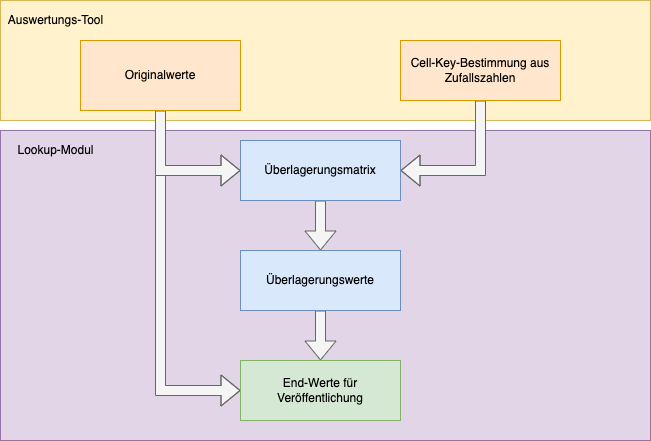
\includegraphics[width=0.59\linewidth]{img/ckm_flow.png}
		\caption{Cell Key Methode - Ablaufdiagramm}
		\label{fig:ckm_flow}
	\end{figure} 
\end{frame}


\begin{frame}{}
	\frametitle{Cell Key Methode - Methodik III}
    \textbf{1 - Erzeugung der Originalwerte mit einem Auswertungs-Tool} 
    %\newline
    %\newline
    %In diesem ersten Schritt werden aus den erhobenen, plausibiliserten statistischen Daten die Veröffentlichungstabellen erstellt. Beispielhaft betrachten wir die %folgende Auswertung. Die darin enthaltenen Werte bezeichnet man als \textbf{Originalwerte}.
    \begin{figure}
		\centering
		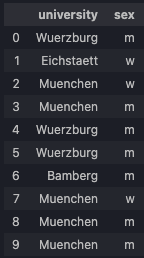
\includegraphics[width=0.2\linewidth]{img/ckm_1.png}
        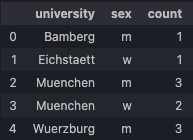
\includegraphics[width=0.25\linewidth]{img/ckm_2.png}
        \caption{Erhobene Mikrodaten (links) und Auswertung mit Originalwerten (rechts)}
	\end{figure} 
\end{frame}


\begin{frame}{}
	\frametitle{Cell Key Methode - Methodik IV}
    \textbf{2 - Cell-Key-Bestimmung aus Zufallszahlen innerhalb des Auswertungs-Tools} 
    \begin{itemize}
        \item Jedem Mikrodatensatz wird eine gleichverteile Zufallszahl $r$, dem sog. \textbf{Record-Key}, mit $r \sim \mathcal{U}(0, 1)$ zugeordnet.
        \item Mit den Record-Keys wird dieselbe Auswertungstabelle wie mit den Originalwerten gebildet. Es ergeben sich also Summen von Record-Keys.
        \item Von diesen Record-Key Summen werden nur die Nachkommastellen betrachtet. Dieser Wert definiert den \textbf{Cell-Key}.
    \end{itemize}
\end{frame}


\begin{frame}{}
	\frametitle{Cell Key Methode - Methodik V}
    \textbf{2 - Cell-Key-Bestimmung aus Zufallszahlen innerhalb das Auswertungs-Tools} 
    \begin{figure}
		\centering
		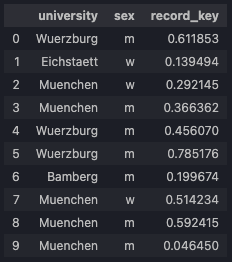
\includegraphics[width=0.25\linewidth]{img/ckm_3.png}
        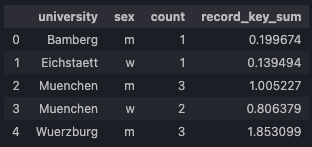
\includegraphics[width=0.3\linewidth]{img/ckm_4.png}
        \caption{Erhobene Mikrodaten mit Record-Key (links) und Auswertung mit Record-Key Summe (rechts)}
	\end{figure} 
    \begin{align*}
        RecordKeySum(Wuerzburg, m) & = 0.611853 + 0.456070 + 0.785176 = 1.853099 \\
        CellKey(Wuerzburg, m) & = 0.853099
    \end{align*}
\end{frame}


\begin{frame}{}
	\frametitle{Cell Key Methode - Methodik VI}
    \textbf{3.1 - Lookup-Modul:  Auslesen der Überlagerungswerte aus der Überlagerungsmatrix}
    \begin{itemize}
        \item Für die Bestimmung eines Überlagerungswerts dient das Paar $(Originalwert, CellKey)$ als Input.
        \item Anhand dieses Wertepaares wird aus der Überlagerungsmatrix der zugehörige Überlagerungswerte abgelesen.
        \item Die Überlagerungsmatrix ist die Lösung eines unterbestimmten nicht-linearen Gleichungsystems, welches aus den Verfahrensparameter und stochastischen Eigenschaften entsteht \cite{Höhne}, \cite{Enderle}.
    \end{itemize}
\end{frame}


\begin{frame}{}
	\frametitle{Cell Key Methode - Methodik VII}
    \textbf{3.1 - Lookup-Modul:  Auslesen der Überlagerungswerte aus der Überlagerungsmatrix}
    Zu den Parametern des Verfahrens zählen \cite{Höhne}:
    \begin{itemize}
        \item Sollen Originalwerte $1$ und $2$ geheimgehalten werden?
        \item Anteil $P_0$ der nicht zu überlagerenden Originalwerte
        \item Die Maximalüberlagerung $d$
        \item Die Standardabweichung der Überlagerungsbeiträge $s$
    \end{itemize}
    mit den stochastischen Eigenschaften \cite{Höhne}:
    \begin{itemize}
        \item Erwartungstreue $E(z) = 0$
        \item Erhalt der Varianz $Var(z) = s^2$
        \item Wahrscheinlichkeitsbedingung $\sum_{n=-d}^{d} P_n = 1$
    \end{itemize}
\end{frame}


\begin{frame}{}
	\frametitle{Cell Key Methode - Methodik VIII}
    \textbf{3.1 - Lookup-Modul:  Auslesen der Überlagerungswerte aus der Überlagerungsmatrix}
    Überlagerungsmatrix aus \cite{Höhne} mit $P_0 = 0.5$, $d = 4$, $s = 2.25$:
    \begin{footnotesize}
    \begin{center}
        \begin{tabular}{ r r r r r r r r r r }
            \textbf{Originalwert} \vline & \textbf{Cell-Key} & & & & & & & & \\ 
            \hline
            $0$ \vline & $0$ & $0$ & $0$ & $0$ & $1$ & $1$ & $1$ & $1$ & $1$ \\
            $1$ \vline & $0$ & $0$ & $0$ & $0.875$ & $0.6875$ & $0.6875$ & $0.9375$ & $1$ & $1$ \\
            $2$ \vline & $0$ & $0$ & $0.3533$ & $0.3533$ & $0.3533$ & $0.9440$ & $0.9970$ & $0.9990$ & $1$ \\
            $3$ \vline & $0$ & $0.1620$ & $0.1620$ & $0.1620$ & $0,6620$ & $0,8560$ & $0,9970$ & $0.9990$ & $1$ \\
            $4$ \vline & $0.0870$ & $0.0870$ & $0.0870$ & $0.1920$ & $0.6920$ & $0.8590$ & $0.9970$ & $0.9990$ & $1$ \\
            $5$ \vline & $0$ & $0$ & $0.1450$ & $0.3270$ & $0.8270$ & $0.8590$ & $0.8930$ & $0.9490$ & $1$ \\
            $6$ \vline & $0$ & $0.0400$ & $0.1500$ & $0.2850$ & $0.7850$ & $0.8600$ & $0.9200$ & $0.9600$ & $1$ \\
            $\geq 7$ \vline & $0.0200$ & $0.0600$ & $0.1450$ & $0.2500$ & $0.7500$ & $0.8550$ & $0.9400$ & $0.9800$ & $1$ \\
            \hline
            \textbf{Überlagerungswert} \vline & $–4$ & $–3$ & $–2$ & $–1$ & $0$ & $1$ & $2$ & $3$ & $4$
        \end{tabular}
    \end{center}
    \end{footnotesize}
\end{frame}


\begin{frame}{}
	\frametitle{Cell Key Methode - Methodik IX}
    \textbf{3.1 - Lookup-Modul:  Auslesen der Überlagerungswerte aus der Überlagerungsmatrix}
    Beispiel: Überlagerungswert für $(\textcolor{red}{Originalwert}, CellKey) = (\textcolor{red}{3}, 0.853099)$
    \begin{footnotesize}
    \begin{center}
        \begin{tabular}{ r r r r r r r r r r }
            \textbf{Originalwert} \vline & \textbf{Cell-Key} & & & & & & & & \\ 
            \hline
            $0$ \vline & $0$ & $0$ & $0$ & $0$ & $1$ & $1$ & $1$ & $1$ & $1$ \\
            $1$ \vline & $0$ & $0$ & $0$ & $0.875$ & $0.6875$ & $0.6875$ & $0.9375$ & $1$ & $1$ \\
            $2$ \vline & $0$ & $0$ & $0.3533$ & $0.3533$ & $0.3533$ & $0.9440$ & $0.9970$ & $0.9990$ & $1$ \\
            $\textcolor{red}{3}$ \vline & $\textcolor{red}{0}$ & $\textcolor{red}{0.1620}$ & $\textcolor{red}{0.1620}$ & $\textcolor{red}{0.1620}$ & $\textcolor{red}{0,6620}$ & $\textcolor{red}{0,8560}$ & $\textcolor{red}{0,9970}$ & $\textcolor{red}{0.9990}$ & $\textcolor{red}{1}$ \\
            $4$ \vline & $0.0870$ & $0.0870$ & $0.0870$ & $0.1920$ & $0.6920$ & $0.8590$ & $0.9970$ & $0.9990$ & $1$ \\
            $5$ \vline & $0$ & $0$ & $0.1450$ & $0.3270$ & $0.8270$ & $0.8590$ & $0.8930$ & $0.9490$ & $1$ \\
            $6$ \vline & $0$ & $0.0400$ & $0.1500$ & $0.2850$ & $0.7850$ & $0.8600$ & $0.9200$ & $0.9600$ & $1$ \\
            $\geq 7$ \vline & $0.0200$ & $0.0600$ & $0.1450$ & $0.2500$ & $0.7500$ & $0.8550$ & $0.9400$ & $0.9800$ & $1$ \\
            \hline
            \textbf{Überlagerungswert} \vline & $–4$ & $–3$ & $–2$ & $–1$ & $0$ & $1$ & $2$ & $3$ & $4$
        \end{tabular}
    \end{center}
    \end{footnotesize}
    Zeile gleich \textcolor{red}{Originalwert} bestimmen.
\end{frame}


\begin{frame}{}
	\frametitle{Cell Key Methode - Methodik X}
    \textbf{3.1 - Lookup-Modul:  Auslesen der Überlagerungswerte aus der Überlagerungsmatrix}
    Beispiel: Überlagerungswert für $(\textcolor{red}{Originalwert}, \textcolor{blue}{CellKey}) = (\textcolor{red}{3}, \textcolor{blue}{0.853099})$
    \begin{footnotesize}
    \begin{center}
        \begin{tabular}{ r r r r r r r r r r }
            \textbf{Originalwert} \vline & \textbf{Cell-Key} & & & & & & & & \\ 
            \hline
            $0$ \vline & $0$ & $0$ & $0$ & $0$ & $1$ & $1$ & $1$ & $1$ & $1$ \\
            $1$ \vline & $0$ & $0$ & $0$ & $0.875$ & $0.6875$ & $0.6875$ & $0.9375$ & $1$ & $1$ \\
            $2$ \vline & $0$ & $0$ & $0.3533$ & $0.3533$ & $0.3533$ & $0.9440$ & $0.9970$ & $0.9990$ & $1$ \\
            $\textcolor{red}{3}$ \vline & $\textcolor{red}{0}$ & $\textcolor{red}{0.1620}$ & $\textcolor{red}{0.1620}$ & $\textcolor{red}{0.1620}$ & $\textcolor{red}{0,6620}$ & $\textcolor{blue}{0,8560}$ & $\textcolor{red}{0,9970}$ & $\textcolor{red}{0.9990}$ & $\textcolor{red}{1}$ \\
            $4$ \vline & $0.0870$ & $0.0870$ & $0.0870$ & $0.1920$ & $0.6920$ & $0.8590$ & $0.9970$ & $0.9990$ & $1$ \\
            $5$ \vline & $0$ & $0$ & $0.1450$ & $0.3270$ & $0.8270$ & $0.8590$ & $0.8930$ & $0.9490$ & $1$ \\
            $6$ \vline & $0$ & $0.0400$ & $0.1500$ & $0.2850$ & $0.7850$ & $0.8600$ & $0.9200$ & $0.9600$ & $1$ \\
            $\geq 7$ \vline & $0.0200$ & $0.0600$ & $0.1450$ & $0.2500$ & $0.7500$ & $0.8550$ & $0.9400$ & $0.9800$ & $1$ \\
            \hline
            \textbf{Überlagerungswert} \vline & $–4$ & $–3$ & $–2$ & $–1$ & $0$ & $\textcolor{blue}{1}$ & $2$ & $3$ & $4$
        \end{tabular}
    \end{center}
    \end{footnotesize}
    \textcolor{blue}{CellKey} kleiner als Spaltenwert bestimmen $\Rightarrow$ Überlagerungswert $ = \textcolor{blue}{1}$.
\end{frame}


\begin{frame}{}
	\frametitle{Cell Key Methode - Methodik XI}
    \textbf{3.2 - Lookup-Modul: Addieren der Überlagerungswerte und Originalwerte}
    \begin{figure}
        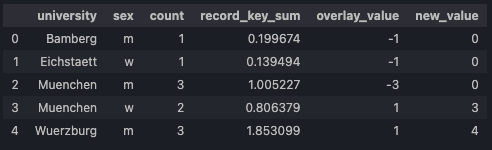
\includegraphics[width=0.7\linewidth]{img/ckm_5.png}
        \caption{Anwendung der CKM auf die Originalwerte}
    \end{figure}
    Originalwerte: \textit{count}, Überlagerungswerte: \textit{overlay value}, End-Werte: \textit{new value}
\end{frame}


%------------------------------------------------
\subsection{Probleme der CKM}

\begin{frame}{}
	\frametitle{Probleme der CKM - Nicht Additivität I}
    \begin{figure}
		\centering
        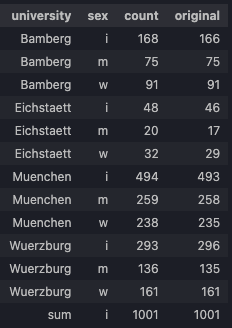
\includegraphics[width=0.25\linewidth]{img/ckm_6.png}
        \caption{Gegenüberstellung von überlagerten Werten mit Originalwerten}
	\end{figure} 
\end{frame}


\begin{frame}{}
	\frametitle{Probleme der CKM - Nicht Additivität II}
    \begin{figure}
		\centering
        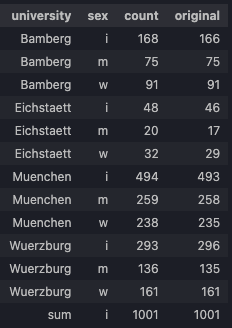
\includegraphics[width=0.25\linewidth]{img/ckm_6.png}
        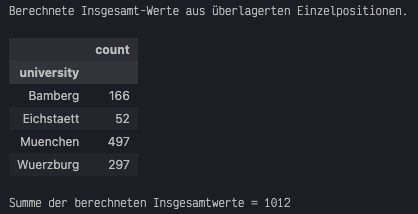
\includegraphics[width=0.55\linewidth]{img/ckm_7.png}
        \caption{Gegenüberstellung von überlagerten Werten mit Originalwerten}
	\end{figure} 
\end{frame}


%------------------------------------------------
\section{Fazit}
%------------------------------------------------

\begin{frame}{}
	\frametitle{Fazit}
    \begin{itemize}
        \item Die CKM ist ein gut \textbf{automatisierbares} Geheimhaltungsverfahren
        \item Es kann \textbf{on top} bei bestehenden Auswertungs-Tools implementiert werden
        \item Es bedarf einer klaren Kommuniktion der besonderen \textbf{Nicht-Additivität} an Außenstehende
        \item Die CKM wird das zentrale Geheimhaltungsverfahren in der \textbf{amtlichen Hochschulstatistik}
        \item Die CKM soll auch beim \textbf{Zensus 2022} für Auswertungen basierend auf Gebäude- und Wohnungsdaten, Haushaltsdaten und Familiendaten angewandt werden \footnotemark \footnotetext[1]{s. \url{https://www.zensus2022.de/DE/Zensusdatenbank/Geheimhaltung.html}}
    \end{itemize}
\end{frame}


%------------------------------------------------
% References
%------------------------------------------------

\begin{frame}
    \frametitle{Literaturverzeichnis}
    \scriptsize{
        \begin{thebibliography}{99} % Beamer does not support BibTeX so references must be inserted manually as below
            %\bibitem[Bronstein, 2020]{Bronstein}  Bronstein, Ilja N., et al. 
            %\newblock Taschenbuch der Mathematik. 11. Auflage, Springer-Verlag, 2020.

            \bibitem[Enderle, 2019]{Enderle} Enderle, Tobias und Meike Vollmar
            \newblock Geheimhaltung in der Hochschulstatistik. \emph{WISTA} | 6, Statistisches Bundesamt (Destatis), Wiesbaden 2019.

            \bibitem[Höhne, 2019]{Höhne} Höhne, Jörg und Julia Höninger
            \newblock Die Cell-Key-Methode – ein Geheimhaltungsverfahren. \emph{Statistische Monatshefte Niedersachsen} 1, 2019.

            \bibitem[Nickl, 2019]{Nickl} Nickl, Andreas
            \newblock Datenschutz, Geheimhaltung, Anonymisierung. \emph{Einführungsfortbildung} Bayerisches Landesamt für Statistik,, Fürth, 2019.

            \bibitem[Rothe, 2015-5]{Rothe-1} Rothe, Patrick
            \newblock Statistische Geheimhaltung – Der Schutz vertraulicher Daten in der amtlichen Statistik - Teil 1: Rechtliche und methodische Grundlagen \emph{Bayern in Zahlen} 5, Bayerisches Landesamt für Statistik, München, 2015.

            \bibitem[Rothe, 2015-8]{Rothe-2} Rothe, Patrick
            \newblock Statistische Geheimhaltung – Der Schutz vertraulicher Daten in der amtlichen Statistik - Teil 2: Herausforderungen und aktuelle Entwicklungen. \emph{Bayern in Zahlen} 8, Bayerisches Landesamt für Statistik, München, 2015.

            \bibitem[Wipke, 2018]{Wipke} Wipke, Mirko
            \newblock Geheimhaltung im Data Warehouse - Prototypische Implementierung von automatisierter Geheimhaltung im Data Warehouse für die amtliche Hochschulstatistik in Bayern. \emph{Bayern in Zahlen} 12, Bayerisches Landesamt für Statistik, Fürth, 2018.

            % Example entry.
            %\bibitem[Smith, 2012]{p3} John Smith (2002)
            %\newblock Title of the publication
            %\newblock \emph{Journal Name} 12(3), 45 -- 678.
        \end{thebibliography}
    }
\end{frame}

%------------------------------------------------

\begin{frame}
    \Huge{\centerline{Zeit für Fragen...}}
    \bigskip
    \bigskip
    \bigskip
    \bigskip

    \normalsize
    \centering
    Folien, \LaTeX \: und Python Code verfügbar auf GitHub \faicon{github} unter:
    \url{https://github.com/JoshuaSimon/Cell-Key-Method}
    \newline
    \newline
    \qrcode{https://github.com/JoshuaSimon/Cell-Key-Method}
\end{frame}

%----------------------------------------------------------------------------------------

\end{document} 